\documentclass[result.tex]{subfiles}

\begin{document}

    \section*{\centering Theory}

    In this chapter we will formalize the reinforcement learning problem mathematically and define the methods to solve our particular reinforcement learning problem.

    \subsection*{Framework}

    To begin the definition of the reinforcement learning problem we first need to define a few fundamental terms that are required in the following formalization. The basic idea is to learn from interactions in order to achieve a goal. The learner is called the \textit{agent} which interacts with the \textit{environment} by performing \textit{actions} in a sequence. The agent is continuously interacting with the environment and it responds based on those interactions in the form of a representation of the \textit{state} of the environment. Not only may the environment change its state, it also give rise to \textit{rewards}, numerical values that the agent is trying to maximize. Figure \ref{fig:agent_env} shows the interactions between the agent and the environment. A complete specification of an environment and how its rewards are determined defines a \textit{task}, which is an instance of a reinforcement learning problem.

    \begin{figure}[H]
        \centering
        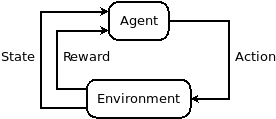
\includegraphics[width=0.6\textwidth]{./images/agent_env}
        \label{fig:agent_env}
        \caption{The agent-environment interaction loop.}
    \end{figure}

    This rather simple framework is actually abstract and flexible enough to be applied in many problems in many different ways. The actions could range from low level controls such as turning the wheels on the car to driving from point A to point B. Similarly, the state could represent current road surface condition to traffic flow in the nearby area. The reward will however always be a single numerical value since we require it to be comparable to be able to determine the best action, the action that will maximize the total amount of reward the agent receives. We will come back to what that means in the following section.

    \subsection*{Markov Decision Process}

    We are going to limit our problem formalization to a special case with discrete time steps, finite state space, finite action space, fully observable state, and episodic tasks. It can be generalized to continuous time steps, infinite state space, infinite action space, partially observable state, and continuing tasks, but is out of scope for this report.

    \subsubsection*{Notation}

    Before continuing with the definition we need to present the most important notation that will be used from now on through the rest of the report.
    \newline
    $\actionspace$: Action space \\
    $\statespace$: State space \\
    $A_t \in \actionspace$: Action at time $t$ \\
    $S_t \in \statespace$: State at time $t$ \\
    $R_t \in \rewardspace$: Reward at time $t$
    \newline
    where $t \in \{ 0, 1, 2, \ldots, T \}$ since we have discrete time steps.

    \subsubsection*{Dynamics}

    We will now formalize the reinforcement learning problem through the \textit{Markov Decision Process} (MDP), in particular \textit{finite} MDP, by sticking to the limitations mentioned above. This formalization assumes that the problem satisfies the \textit{Markov property} which means that the one-step dynamics of the problem holds the following

    \begin{align*}
        Pr(S_{t + 1} = \nextstate, R_{t + 1} = r | S_0, A_0, R_1, \ldots, S_{t - 1}, A_{t - 1}, R_t, S_t, A_t) = Pr(S_{t + 1} = \nextstate, R_{t + 1} = R | S_t, A_t),
    \end{align*}

    which in words says that the future state and reward is independent of the past actions, states, and rewards given the current action and state. To simplify this formula we write it as

    \begin{align*}
        p(\nextstate, r | s, a) &=
        Pr(S_{t + 1} = \nextstate, R_{t + 1} = r | S_t = s, A_t = a)
    \end{align*}

    and it completely specifies the dynamics of the finite MDP. We can compute anything we might want to get from it such as the the \textit{state-transition probabilities} and the \textit{expected reward} for state-action pairs

    \begin{align*}
        p(\nextstate | s, a) &=
        \sum_r p(\nextstate, r | s, a), \\
        r(s, a) &=
        \expectation \left[ R_{t + 1} | S_t = s, A_t = a \right] =
        \sum_{r \in \rewardspace} r \sum_{\nextstate \in \statespace} p(\nextstate, r | s, a).
    \end{align*}

    \begin{align*}
        \pi(a | s) &= Pr(A_t = a | S_t = s)
    \end{align*}

    \subsubsection*{Expected Reward}

    \begin{align*}
        r(s, a) &=
        \mathbb{E} \left[ R_{t + 1} \bigg\rvert S_t = s, A_t = a \right] =
        \sum_r r \sum_{\nextstate} p(\nextstate, r | s, a) \\
        r(s, a, \nextstate) &=
        \mathbb{E} \left[ R_{t + 1} \bigg\rvert S_t = s, A_t = a, S_{t + 1} = \nextstate \right] =
        \frac{\sum_r r p(\nextstate, r | s, a)}{p(\nextstate | s, a)}
    \end{align*}


    \subsubsection*{State-Value Function}

    \begin{align*}
        v_{\pi}(s) &= \mathbb{E} \left[ \sum_{k=0}^{\infty} \gamma^k R_{t + k + 1} \bigg\rvert S_t = s \right] \\
        &= \sum_a \pi(a | s) \sum_{\nextstate, r} p(\nextstate, r | s, a) \left[ r + \gamma v_\pi(\nextstate) \right]
    \end{align*}

    \subsubsection*{Action-Value Function}

    \begin{align*}
        q_{\pi}(s, a) = \mathbb{E} \left[ \sum_{k=0}^{\infty} \gamma^k R_{t + k + 1} \bigg\rvert S_t = s, A_t = a \right]
    \end{align*}

    \subsection*{Temporal Difference Learning}

    \textit{Temporal Difference} (TD) learning is a learning methodology that learns directly from raw experience without a model of the environment's dynamics. It update new estimates partially on previous estimates without waiting for the final outcome, i.e. bootstraps estimates. The algorithms, or learning methods, that have been used in this paper are all based on TD learning and will be described below.

    \subsubsection*{Q-Learning}

    Q-learning is a widely used algorithm that was developed by \textbf{(Watkins, 1989)} and is heavily used to day combined with the emergence of neural networks \textbf{deep reinforcement learning, atari}. It is defined as

    \begin{align*}
        Q(S_t, A_t) &=
        Q(S_t , A_t) +
        \alpha \left[
        R_{t + 1} +
        \gamma \max_a Q(S_{t + 1}, a) - Q(S_t, A_t).
        \right]
    \end{align*}

    It is a so called \textit{off-policy} method which is indicated by the $\max_a$ operation. That means it uses a greedy algorithm to estimate the return at the next step rather than following its current policy, therefore is off its own policy. The Sarsa algorithm described below is an example of a on-policy method.

    \subsubsection*{Sarsa}

    \begin{align*}
        Q(S_t, A_t) &=
        Q(S_t , A_t) +
        \alpha \left[
        R_{t + 1} +
        \gamma Q(S_{t + 1}, A_{t + 1}) - Q(S_t, A_t)
        \right]
    \end{align*}

    \subsubsection*{Expected Sarsa}

    \begin{align*}
        Q(S_t, A_t) &=
        Q(S_t , A_t) +
        \alpha \left[
        R_{t + 1} +
        \gamma \mathbb{E} \left[ Q(S_{t + 1}, A_{t + 1}) | S_{t + 1}
        \right] -
        Q(S_t, A_t)
        \right] \\
        &=
        Q(S_t , A_t) +
        \alpha \left[
        R_{t + 1} +
        \gamma \sum_a \pi (a | S_{t + 1}) Q(S_{t + 1}, a) -
        Q(S_t, A_t)
        \right]
    \end{align*}

    \subsection*{Other Learning Methods}

    \subsubsection*{Dynamic Programming}

    \subsubsection*{Monte Carlo}

    \subsubsection*{Extensions}

\end{document}
